\subsubsection{الگوی \lr{Protected Single Channel}}
\label{archSafeProtectSingleChSec}
\begin{RTL}
\lr{redundancy} کامل در سیستم‌هایی که امنیت در آن‌ها حیاتی است،
پرهزینه است، هم در تکرار سخت‌افزار و هم در توسعه آن.
این الگو \cite{ref4}
یک جایگزین سبک برای افزایش ایمنی و قابلیت اطمینان است که با افزودن
چک‌های اضافی و مقداری سخت‌افزار اضافی این کار را انجام می‌دهد.
این الگو از یک کانال برای حسگر و تحریک استفاده می‌کند و خطاهای گذرا را
شناسایی و مدیریت می‌کند، اما خطاهای پایدار را نمی‌تواند مدیریت کند.
این رویکرد از نظر هزینه‌های تکراری و توسعه مقرون به صرفه است و برای سیستم‌هایی
که نیاز به عملکرد در حضور خطاهای پایدار ندارند یا حساس به هزینه هستند،
مناسب است. با این حال، به دلیل نقاطی که یک خطای منفرد می‌تواند باعث
از دست رفتن کل سیستم شود، برای همه سیستم‌های مرتبط با ایمنی مناسب نیست.
این الگو مشابه \nameref{safeProtSingleChSec} است که
در \cite{ref1} آورده شده‌است؛ با این تفاوت که در اینجا در ابعاد معماری
تعریف شده.
\end{RTL}
\begin{figure}[h!]
\centering
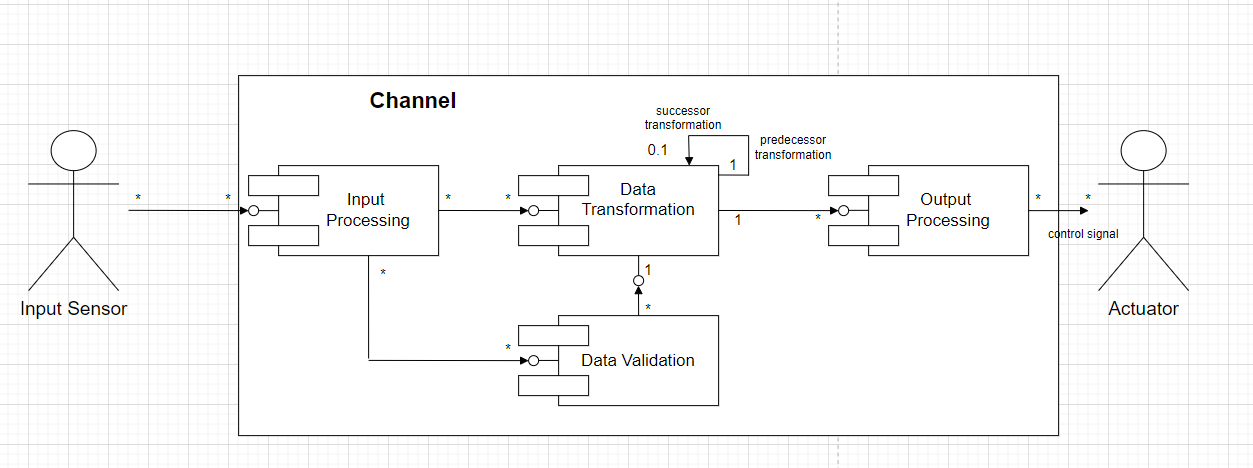
\includegraphics[scale=0.5]{images/second/protectedSingle.png}
\caption{ساختار الگوی \lr{Protected Single Channel}}
\end{figure}